\documentclass{article}
\usepackage[landscape]{geometry}
\usepackage{url}
\usepackage{multicol}
\usepackage{amsmath}
\usepackage{esint}
\usepackage{amsfonts}
\usepackage{tikz}
\usetikzlibrary{decorations.pathmorphing}
\usepackage{amsmath,amssymb}
\usepackage{physics}
\usepackage{colortbl}
\usepackage{xcolor}
\usepackage{mathtools}
\usepackage{amsmath,amssymb}
\usepackage{enumitem}
\usepackage{graphicx}
\makeatletter

\newcommand*\bigcdot{\mathpalette\bigcdot@{.5}}
\newcommand*\bigcdot@[2]{\mathbin{\vcenter{\hbox{\scalebox{#2}{$\m@th#1\bullet$}}}}}
\makeatother

\title{130 Cheat Sheet}
\usepackage[brazilian]{babel}
\usepackage[utf8]{inputenc}

\advance\topmargin-.8in
\advance\textheight3in
\advance\textwidth3in
\advance\oddsidemargin-1.5in
\advance\evensidemargin-1.5in
\parindent0pt
\parskip2pt
\newcommand{\hr}{\centerline{\rule{3.5in}{1pt}}}
%\colorbox[HTML]{e4e4e4}{\makebox[\textwidth-2\fboxsep][l]{texto}
\begin{document}

\begin{center}{\huge{\textbf{PHYS 200 Midterm 2 Cheat Sheet}}}\\
\end{center}
\begin{multicols*}{3}

\tikzstyle{mybox} = [draw=black, fill=white, very thick,
    rectangle, rounded corners, inner sep=10pt, inner ysep=10pt]
\tikzstyle{fancytitle} =[fill=black, text=white, font=\bfseries]

%------------ Heating ---------------
\begin{tikzpicture}
\node [mybox] (box){%
    \begin{minipage}{0.3\textwidth}
    $$E=\gamma mc^2, \vert \vec{p} \vert = \gamma mv \to E^2 = m^2 c^4 + p^2 c^2$$
    $$\vec{F} = \frac{d\vec{p}}{dt}$$
    LMatrix : $$\begin{bmatrix} \gamma & -\beta\gamma & 0 & 0 \\ -\beta\gamma & \gamma & 0 & 0 \\ 0 & 0 & 0 & 0 \\ 0 & 0 & 0 & 0 \end{bmatrix}$$

    \end{minipage}
};
%------------ Heating Header ---------------------
\node[fancytitle, right=10pt] at (box.north west) {Relativistic Dynamics};
\end{tikzpicture}

%------------ Mixing ---------------
\begin{tikzpicture}
\node [mybox] (box){%
    \begin{minipage}{0.3\textwidth}
      1. massless\\
      2. no rest frame\\
      3. always move at $c$ (in all frames)\\
      4. $E=pc=hc/\lambda$, definite energy and momentum, related to \textbf{wavelength}
    \end{minipage}
};
%------------ Mixing Header ---------------------
\node[fancytitle, right=10pt] at (box.north west) {Photons};
\end{tikzpicture}

%------------ Inner Product Spaces ---------------
\begin{tikzpicture}
\node [mybox] (box){%
    \begin{minipage}{0.3\textwidth}
      1. Energy, momentum is always conserved $\rightarrow$ mass doens't have to be, can convert mass into KE\\
      2. Fusion: 2 light things $\rightarrow$ heavy thing + E \\
      3. Fission: 1 heavy thign $\rightarrow$ 2 (or more) lighter things + E \\
      4. Since stable is less energy state, we exert energy to go to stable state  \\
      5. In hydrogen atom $m_H = m_e + m_p - BE \to m_H  < m_e + m_p$ 
      
    \end{minipage}
};
%------------ Inner Product Space Header ---------------------
\node[fancytitle, right=10pt] at (box.north west) {Mass};
\end{tikzpicture}

%------------ Gram-Schmidt Content ---------------
\begin{tikzpicture}
\node [mybox] (box){%
    \begin{minipage}{0.3\textwidth}
    1. Move to center of mass frame (where stationary object decays). \\ 
    2. Compute momentum $\&$ energy, using LT revert back to original frame (be careful of sign).
    \end{minipage}
};
%------------ Gram-Schmidt Header ---------------------
\node[fancytitle, right=10pt] at (box.north west) {Particle decay, how to solve for diff frames};
\end{tikzpicture}
%------------ Variation of Parameters Content ---------------------
\begin{tikzpicture}
\node [mybox] (box){%
    \begin{minipage}{0.3\textwidth}
      $$\lambda' - \lambda = \frac{h}{m_e c}(1-\cos{\theta})$$
      1. $m$ is dependent on the object we are striking the photon to.\\
      2. Don't forget unit conversions.
    \end{minipage}
};
%------------ Variation of Parameters Header ---------------------
\node[fancytitle, right=10pt] at (box.north west) {Compton Scattering};
\end{tikzpicture}

\begin{tikzpicture}
\node [mybox] (box){%
    \begin{minipage}{0.3\textwidth}
      $$\vec{E_0}\cos{kx-\omega t + \psi} \hspace{.2in} (k = 2\pi / \lambda , \omega = 2\pi f)$$  

\end{minipage}
};
%------------ ODE Header ---------------------
\node[fancytitle, right=10pt] at (box.north west) {Classical view};
\end{tikzpicture}

%------------ Series Solution Content ---------------
\begin{tikzpicture}
\node [mybox] (box){%
    \begin{minipage}{0.3\textwidth}
        \end{minipage}
};
%------------ Series Solution Header ---------------------
\node[fancytitle, right=10pt] at (box.north west) {Classical view continued};
\end{tikzpicture}

%------------ Systems of ODE Content ---------------
\begin{tikzpicture}
\node [mybox] (box){%
    \begin{minipage}{0.3\textwidth}
    1. $c=hf$ \\ 
    2. Energy is proportional to $E_0^2,B_0^2$ \\ 
    3. Intensity $\propto (E_0)^2$ a.k.a Probability $\propto (E_0)^2 \text{ and } I$
    4. Intensity = energy / (area * time), not dependent on frequency of light \\
    5. If intensity increase, it is related to the number of photons
    \end{minipage}
};
%------------ Systems of ODE Header ---------------------
\node[fancytitle, right=10pt] at (box.north west) {Classical view continued};
\end{tikzpicture}

%------------ Exponentiation Content ---------------
\begin{tikzpicture}
\node [mybox] (box){%
    \begin{minipage}{0.3\textwidth}
    1. $E_\gamma = hf$ \\ 
    2. $KE_\text{max} = hf - W$ \\ 
    3. $W$ is same unless metal changes \\ 
    4. $eV_\text{stop} = KE_\text{max} = hf - W$ \\ 
    5. If retarding potential applied, it is not that electrons are not ejected,  
    it is because some ejected electrons can't make through
    \end{minipage}
};
%------------ Spring-Mass Header ---------------------
\node[fancytitle, right=10pt] at (box.north west) {Photo Electric Effect};
\end{tikzpicture}
\
%------------ Laplace Transforms Content ---------------
\begin{tikzpicture}
\node [mybox] (box){%
    \begin{minipage}{0.3\textwidth}
    1. Compton Scattering \\ 2. Photoelectric: not existence of effect, rather it is effect of retarding potential, nature that it's a hit or a miss and photon disappers after hitting 
    \\ 3. Blackbody radiation: When wavelength is low, radiation is not infinite. (related to cost of ejecting a high energy particle) 
  \end{minipage}
};
%------------ Laplace Transforms Header ---------------------
\node[fancytitle, right=10pt] at (box.north west) {QM effect of light};
\end{tikzpicture}
%------------ Gaussian Integral Content ---------------------
\begin{tikzpicture}
\node [mybox] (box){%
    \begin{minipage}{0.3\textwidth}
    1. Photon / electron has a probability of hitting part of screen \\ 
    2. Somehow each particle knows diffraction pattern. Somehow each particle passes through both slits at the same time \\ 
    3. We don't know till measure \\ 
    4. hit screen at certain point (particle behav.), interference (with itself) pattern (wave behaviour) \\ 
    5. After measurement (position checked), position collapses and has definite position. 
    6. Before measurement, no position is known (only a probability distribution is known)
    \end{minipage}
};
%------------ Gaussian Integral Header ---------------------
\node[fancytitle, right=10pt] at (box.north west) {Diffraction pattern};
\end{tikzpicture}
%------------ Complex Numbers Content ---------------------
\begin{tikzpicture}
\node [mybox] (box){%
    \begin{minipage}{0.3\textwidth}

      1. Intensity $\propto$ E-field squared, thus probability $\propto$ wave amplitude squared \\ 
      2. $P(x) = \vert \psi(x) \vert ^2 = \psi(x) \bar{\psi(x)}$
	\end{minipage}
};
%------------ Gaussian Integral Header ---------------------
\node[fancytitle, right=10pt] at (box.north west) {Probability};
\end{tikzpicture}

%------------ Vector Spaces ---------------
\begin{tikzpicture}
\node [mybox] (box){%
    \begin{minipage}{0.3\textwidth} 
    1. Measurement : process through which observales is determined / recorded (position, momentum recorded) \\ 
    2. Eigenstate : A quantum state with 100 percent certainty  \\
    3. Quamtum superposition : Combination of different eigenstates with complex coefficients \\ 
    4. State : complete description of properties at some moment in time
  \end{minipage}
};
%------------ Vector Space Header ---------------------
\node[fancytitle, right=10pt] at (box.north west) {Terminlogies};
\end{tikzpicture}

\begin{tikzpicture}
\node [mybox] (box){%
    \begin{minipage}{0.3\textwidth} 
      1. $\sum_{\forall x}c(x) \ket{x} \equiv \int_{-\infty}^{\infty}c(x) \ket{x} dx$ \\ 
      2. $\ket{\psi(x)} = \int_{\infty}^{\infty} \psi(x) \ket{x}dx$  \\ 
      3. After measurement, state changes to appropriate eigen state \\ 
      4. If repeated measurement right after, get same result (system still in that eigenstate) \\ 
      5. If asked about diff measurement, we have to change basis i.e. new eigenstate \\ 
      6. Given $a_1\ket{x_1} + a_2\ket{x_2}$, a particle DOES NOT have a definite state.
    \end{minipage}
};
%------------ Vector Space Header ---------------------
\node[fancytitle, right=10pt] at (box.north west) {QM / Measurements};
\end{tikzpicture}

\begin{tikzpicture}
\node [mybox] (box){%
    \begin{minipage}{0.3\textwidth} 
      1. $\ket{\theta} = \cos{\theta} \ket{0} + \sin{\theta} \ket{90}$ \\ 
      2. probability transmission : $\cos^2{\theta}$ \\ 
      3. probability absorbed : $\sin^2{\theta}$ \\ 
      4. In case of $\ket{\phi} = a \ket{x} + b \ket{y}$, when getting probability need to normalize $\vert a\vert ^ 2+ \vert b \vert ^2 = 1$
    \end{minipage}
};
%------------ Vector Space Header ---------------------
\node[fancytitle, right=10pt] at (box.north west) {Polarisation};
\end{tikzpicture}

\begin{tikzpicture}
\node [mybox] (box){%
    \begin{minipage}{0.3\textwidth} 
    1. For any particle, $pc = hc / \lambda \implies p = h / \lambda$. \\ 
    2. Use $e^{i2\pi p x / h}$ \\ 
    3. $\psi(x) = \frac{1}{\sqrt{h}} \int{\tilde{\psi}(p) e^{ipx/ \hbar}dp}$ \\ 
    4. $\tilde{\psi(p)}=\frac{1}{\sqrt{h}} \int{\psi(x)e^{-ipx/\hbar}dx}$ \\ 
  5. For post-measurement, $\psi(x) = e^{ip_0 x/\hbar},\tilde{\psi}(p)= e^{-ip x_0 /\hbar}$, cannot be properly normalized \\
    6. $\psi(R,t) = e^{2\pi i (R/ \lambda - ft)}, \hspace{.1in} R \approx D + \frac{Y^2}{2D}$ \\ 
    7. $\langle  x \rangle = \int_{-\infty}^{\infty} xP(x)dx= \int_{-\infty}^{\infty} x \vert \Psi(x) \vert^2 dx$ \\ 
    8. $\hbar = \frac{h}{2\pi}$, heisenberg uncertainty: $\Delta x \Delta p \geq \hbar / 2$
  \end{minipage}
};

%------------ Vector Space Header ---------------------
\node[fancytitle, right=10pt] at (box.north west) {De bregolie wave length};
\end{tikzpicture}

\pagebreak


\begin{tikzpicture}
\node [mybox] (box){%
    \begin{minipage}{0.3\textwidth} 
      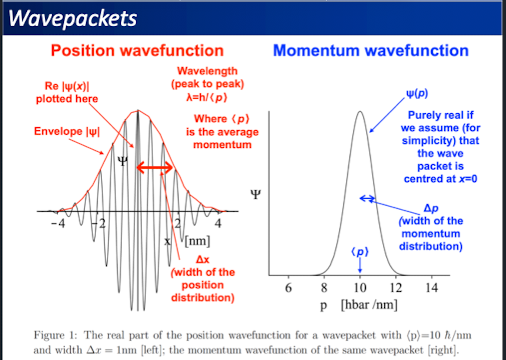
\includegraphics[width=\linewidth]{wavepacketimg.png} \\ 
      1. Wavepackets are needed to localize real wavefunctions (which are not as shown above) \\
      2. The narrower the wavepacket in position, wider range of frequencies, wider momentum wavefunction \\ 
      3. The narrower the wavepacket in momentum, the wider position wavefunction. \\ 
      4. $\langle p \rangle = \int_{-\infty}^{\infty} p \vert \tilde{\Psi}(p) \vert^2 dp$ \\ 
      5. $ (\Delta p)^2 = \int_{-\infty}^{\infty} (p - \langle p \rangle )^2 \vert \tilde{\Psi}(x) \vert^2 dp$
    \end{minipage}
};

%------------ Vector Space Header ---------------------
\node[fancytitle, right=10pt] at (box.north west) {Wave Packets};
\end{tikzpicture}




\begin{tikzpicture}
\node [mybox] (box){%
    \begin{minipage}{0.3\textwidth} 
      $$c= 3.00 \times 10^8 \text{ms}^{-1}, \hspace{.3in} e = 1.60 \times 10^{-19}C $$ $$ h = 6.626 \times 10^{-34} \text{Js}$$
      $$m_e = 9.11 \times 10^{-31} \text{kg} , \hspace{.2in} m_p = 1.67 \times 10^{-27} \text{kg}$$
      $$m_{\pi_0} = 2.406 \times 10^{-28}\text{kg },u_x' = \frac{u_x - v}{1 - u_xv/c^2}$$
      $$\mathbf{P} = (\gamma(u)mc, \gamma(u)m\vec{u})= (E/c,\vec{p})$$
      $$1J = 6.242\times 10^{18}eV$$ \\ 
      1. Bound system has binding energy. Stable so low E. \\ 
      2. Bound system's mass is less than the sum of the masses of the components. \\ 
      3. Unstable bound system has sum of masses heavier than its components. \\ 
      4. Having half vertical and half horizontal polarized light is different from $\frac{1}{\sqrt{2}} \ket{0} + \frac{1}{\sqrt{2}} \ket{90}$ \\ 
      5. Bright fringes : $\frac{dY}{D} = m\lambda$, $d:\text{slit size}, D: \text{ Distance to screen}, Y: \text{ Height}$
    \end{minipage}
};

%------------ Vector Space Header ---------------------
\node[fancytitle, right=10pt] at (box.north west) {Constants, Formulae and others};

\end{tikzpicture}

\begin{tikzpicture}
\node [mybox] (box){%
    \begin{minipage}{0.3\textwidth} 
    1. A wavefunction of a moving free particle with a well defined momentum is simply a travelling wave \\ 
    $$e^{(i/\hbar)(px-Et)}$$
    2. $E= 1/2mv^2 = p^2/2m$ (non-relativistic) \\
    3. Time evolution for each component in a quamtum superposition happens independently
    
    \end{minipage}
};

%------------ Vector Space Header ---------------------
\node[fancytitle, right=10pt] at (box.north west) {Time evolution};


\end{tikzpicture}



\end{multicols*}
\end{document}


Contact GitHub API Training Shop Blog About
© 2016 GitHub, Inc. Terms Privacy Security Status Help
